%you can change blue to red or blackandwhite
\documentclass[blue]{beamer}
%theme selection
\usetheme{Warsaw}
%use necessary packages
\usepackage{array}
\usepackage{graphicx}

%presentation details
\title[A study of BFT algorithms]{A study of Byzantine fault-tolerant algorithms}
\subtitle{}
\author{Author goes here}
\institute[webpage]{Institute \\ Department}
\date{Date goes here}
\begin{document}

%title page
\begin{frame}
\titlepage
\end{frame}

%table of contents
\begin{frame}
\frametitle{Table of Contents}
%use this line instead of the one bellow to highlight the current section in the table of contents
%\tableofcontents[currentsection]
\tableofcontents
\end{frame}

%section
\section{Introduction}

%quote
\begin{frame}
 \frametitle{Fault Tolerance}
\noindent
 \textit{``A distributed system is one in which the failure of a computer you didn't even know existed can render your own computer unusable.''}
 \\Leslie Lamport
\end{frame}

%item list
\begin{frame}
 \frametitle{Failure models}
\begin{itemize}
 \item Crash failures
 \item Omission failures
 \item Timing failures
 \item Response failures
 \item Byzantine (arbitrary) failures
\end{itemize}
\end{frame}

%numbered list
\section{Algorithms}
\begin{frame}
 \frametitle{Algorithms}
\begin{enumerate}
 \item Practical Byzantine Fault Tolerance
 \item Query/Update (Q/U)
 \item BFT2F
 \item Zyzzyva
 \item CheapBFT
\end{enumerate}
\end{frame}

%numbered list - show items step by step
%important! don't forget to add the "handout" option to the documentclass if you are going to print the slides!
\begin{frame}
 \frametitle{Algorithms - Step by step}
\begin{enumerate}
 \item<1-> Practical Byzantine Fault Tolerance
 \item<2-> Query/Update (Q/U)
 \item<3-> BFT2F
 \item<3-> Zyzzyva
 \item<4-> CheapBFT
\end{enumerate}
\end{frame}

%figure
\begin{frame}
 \frametitle{Practical Byzantine Fault Tolerance}
\begin{figure}
\begin{center}
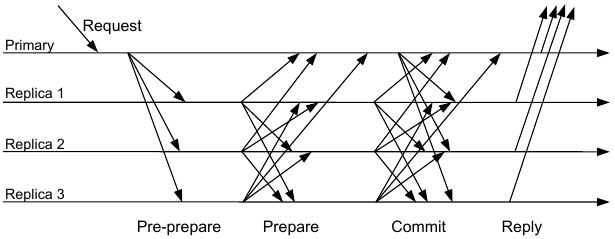
\includegraphics[width=4.5in]{protocol}\\
\end{center}
\end{figure}
\end{frame}

%framed text
\begin{frame}
\frametitle{Framed text}
\begin{block}{Block}
Block text
\end{block}
\begin{example}{Example}
text
\end{example}
\begin{alertblock}{Alert block}
Alert block text
\end{alertblock}
\end{frame}

\section{Conclusion}

%end frame
\begin{frame}
 \frametitle{End of Presentation}
Questions?
\end{frame}


\end{document}
